\section{Отбор признаков}

\begin{Отбор признаков}
Основныя цели отбора признаков - уменьшение размерности задачи, а также выявление и отбрасывание признаков,
 не несущих полезной для решения задачи информации. Снижение размерности также ведёт к уменьшению времени обучения алгоритмов и уменьшению размера, занимаемого тренировочной выборкой.
 \par
Для рассматриваемого набора данных большая часть переменных не меняет значений на всех объектах выборки,
 поэтому все признаки с нулевой дисперсией были отброшены. В результате размерностьзадачи была сокращена
 с 4125 до около 230 переменных (227-229 в зависимости от канала). Такая ситуация произошла из-за использования схемы Bag of Words при создании датасета. 
 \subsection{PCA}
 \begin{PCA}
 Для дальнейшего уменьшения количества признаков использовался метод главных компонент
 (principal component analysis или PCA). Этот метод позволяет снизить размерность оптимальным с точки зрения некоторого критерия образом. Рассмотрим его подробнее.
 \par
 Постановка задачи, решаемой в методе PCA звучит следующим образом: найти линейное многообразие заданной 
 размерности, сумма квадратов расстояний до которого от данной системы точек минимальна. Стоит обратить внимание на то, что информация о принадлежности точек к какому-либо классу здесь не учитывается.
 Пусть \( X_i \subseteq \mathbb{R}^n, i=\overline{1,m} \) --- набор произвольных векторов. Требуется найти векторы \(v_0\ldots v_d\subseteq \mathbb{R}^d, \Vert v_j \Vert = 1, v_i \bot v_j, j \neq  i, d \leq n\), задающие линейное многообразие \(L\) так, чтобы \(
 \sum_{i=1}^{m} dist^2(X_i, L) = \sum_{i=1}^{m}\Vert X_i - v_0 - \sum_{j=1}^k\langle X_i - v_0; v_j\rangle\ v_j \Vert\rightarrow min\) В качестве редуцированных данных выступают проекции векторов \( X_i\) на многообразие \(L\). 
 
 
 
 \subsection*{Результаты применения PCA}
 \begin{Результаты применения PCA}
 Лучшие результаты при уменьшении размерности с помошью PCA показал алгоритм random forest.
 \begin{figure} \centering 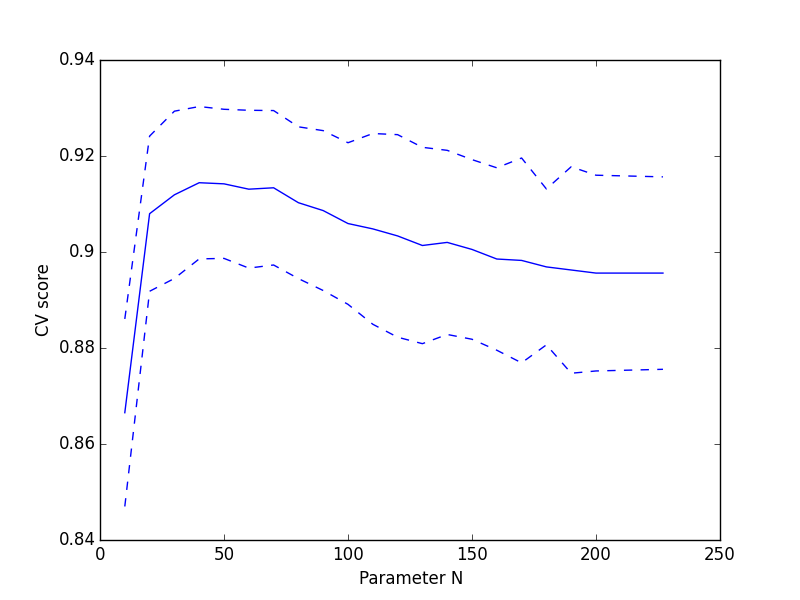
\includegraphics[width=1\textwidth]{images/randforest_NDTV_PCA.png} \caption{Random forest on NDTV } \label{fig:image} \end{figure}
 При одновременном улучшении результата кроссвалидации практически линейно уменьшается время обучения алгоритма.
  \begin{figure} \centering 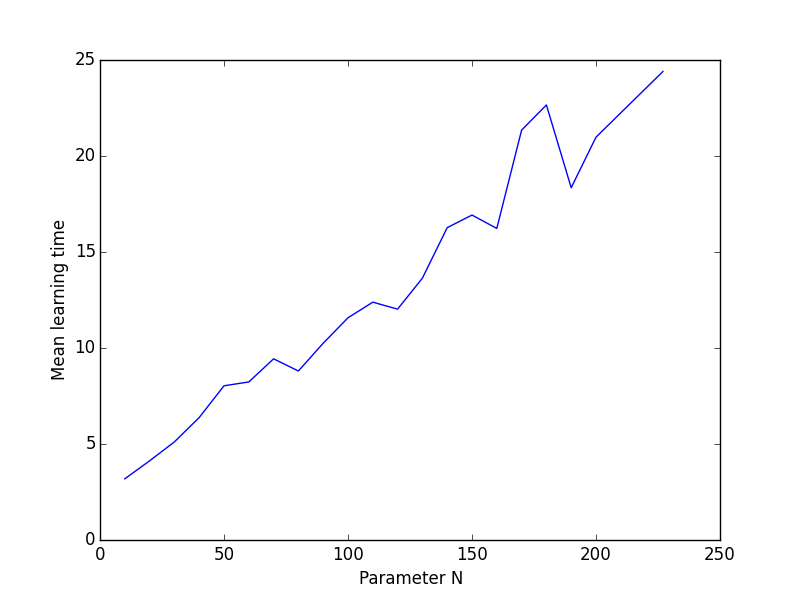
\includegraphics[width=1\textwidth]{images/randforest_NDTV_PCA_time.png} \caption{Random forest on NDTV train time} \label{fig:image} \end{figure}
  Применение PCA в сочетании с LDA не дало результата в плане улучшения качества предсказания. Время обучения также уменьшается линейно.
  \begin{figure} \centering 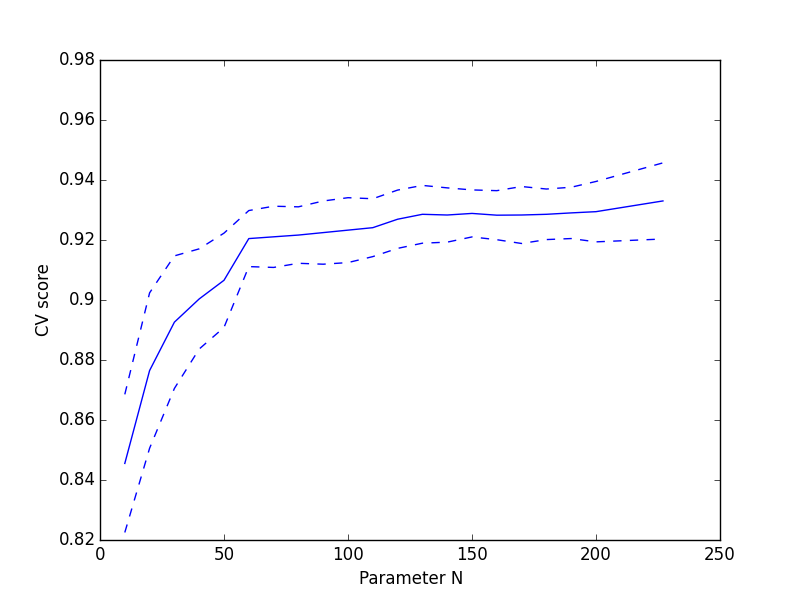
\includegraphics[width=1\textwidth]{images/LDA_NDTV_PCA.png} \caption{LDA on NDTV } \label{fig:image} \end{figure}
  \begin{figure} \centering 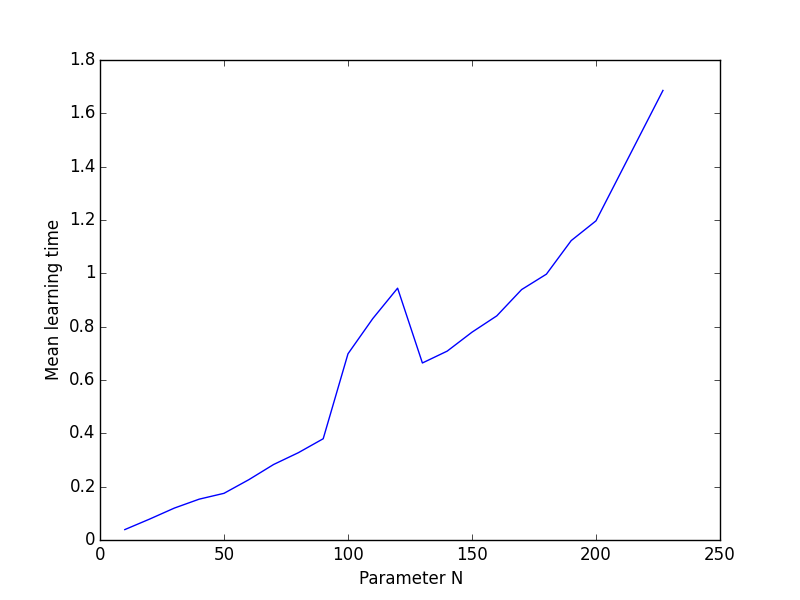
\includegraphics[width=1\textwidth]{images/LDA_NDTV_PCA_time.png} \caption{LDA on NDTV train time} \label{fig:image} \end{figure}
  \par
  
  
